\documentclass[10pt,a4paper]{article}
\usepackage[utf8]{inputenc}
\usepackage[spanish,activeacute]{babel}
\usepackage{a4wide}
\usepackage{amsmath}
\usepackage{amsthm}
\usepackage{amsfonts}
\usepackage{graphicx}
\usepackage{tikz}
\usepackage{tkz-graph}
\usepackage{todonotes}
%\usepackage[lined, ruled, linesnumbered]{algorithm2e}
\usepackage[lined, ruled, linesnumbered]{algorithm2e}
\usepackage{caption}	% Para agregar captions de table a entornos tabular
\usepackage{float}

\graphicspath{{imagenes/}}

\newtheorem{teo}{Teorema}[section]
\newtheorem{prop}{Proposición}[section]
\newtheorem{lema}{Lema}[section]

\theoremstyle{remark}
\newtheorem{obs}{Observación}[section]

\theoremstyle{definition}
\newtheorem{defi}{Definición}[section]

\newcommand{\twodots}{\cdot\cdot\hspace{0.75mm}}

\begin{document}
	\hfill 
\includegraphics[scale = 0.75]{imagenes/logo_dc.jpg}~\\[0.25cm]

\begin{center}
	\textbf{\Large Metamorfosis de Im'agenes Vectorizada}\\[1cm]
	{\large Guido Tagliavini Ponce\\[0.15cm]}
	Universidad de Buenos Aires\\[0.15cm]
	\texttt{guido.tag@gmail.com}\\[1cm]
\end{center}
\rule{\linewidth}{0.2mm}

	\tableofcontents
	\section{Abstract}

Presentamos una vectorizaci'on del algoritmo de metamorfosis de im'agenes de Beier y Neely \cite{beier92}, utilizando las extensiones SIMD de la arquitectura x86-64 de Intel. Comparamos esta implementaci'on contra una versi'on del mismo algoritmo en lenguaje C, compilada con el flag -O3 del compilador de Intel (Intel\textregistered Parallel Studio XE). Las mediciones indican que nuestra versi'on es 11 veces m'as r'apida.
	\section{Introducci'on}

La metamorfosis de im'agenes (en ingl'es, \textit{image morphing}) es una t'ecnica para transformar una imagen (la \textit{imagen origen}) en otra (la \textit{imagen destino}). Esta t'ecnica ha sido ampliamente utilizada en el 'ambito de la industria cinematogr'afica. Un ejemplo can'onico de su aplicaci'on puede verse en el video de la canci'on \textit{Black or White} de Michael Jackson, en el cual hay una secuencia de transformaciones entre las caras de personas de muy distintas caracter'isticas.

Diversos algoritmos para realizar esta metamorfosis han sido desarrollados, siendo el m'as b'asico aquel conocido como \textit{cross-dissolving}, que consiste en hacer desaparecer la imagen origen a medida que se hace aparecer la imagen destino, de forma gradual, creando un efecto de disoluci'on de ambas im'agenes. Concretamente, esta t'ecnica consiste en interpolar de a pares los colores de los p'ixeles de la imagen origen con los de la imagen destino, para luego variar el valor de la interpolaci'on a lo largo del tiempo.

\begin{figure}[H]
	\begin{center}
		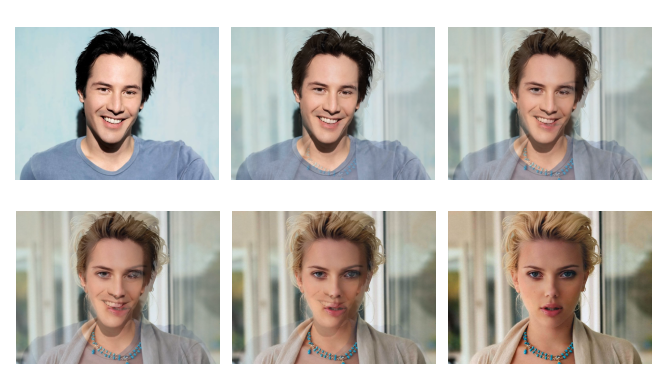
\includegraphics[scale=0.65]{imagenes/dissolving.png}
	\end{center}		
	\caption{Cross-dissolving}
	\label{fig1}
\end{figure}

Esta t'ecnica no resulta satisfactoria, puesto que la transformaci'on no es natural, en el sentido de que no sugiere que lo que ocurre es una metamorfosis. Esto se debe a que las caracter'isticas de la imagen origen no se transforman naturalmente en ciertas otras caracter'isticas de la imagen destino. Por esta raz'on, las t'ecnicas m'as elaboradas de image morphing emplean la deformaci'on de im'agenes (en ingl'es, \textit{image warping}) acompa\~{n}ado de un cross-dissolving, para obtener esa naturalidad buscada en la transformaci'on. La principal diferencia entre los distintos m'etodos de morphing est'a en la forma en que se mapean las caracter'isticas de la imagen origen en las de la imagen destino.

En este trabajo nos concentramos en la t'ecnica desarrollada por Beier y Neely, presentada en \cite{beier92}, que realiza el mapeo de caracter'isticas a trav'es de segmentos dirigidos (l'ineas rectas con principio, fin y sentido) en la imagen origen asociados a segmentos dirigidos en la imagen destino. Esto no s'olo determina c'omo deben ser transformados los puntos sobre esos segmentos, sino que tambi'en dan informaci'on sobre la transformaci'on de los puntos que los rodean. Implementamos una versi'on de este m'etodo basada en instrucciones SIMD, y la comparamos contra una versi'on tradicional, que realiza el procesamiento en serie, ganando, la primera, en t'erminos de tiempo de ejecuci'on, por un amplio margen. No tenemos registro de ninguna publicaci'on sobre una implementaci'on de este tipo, ni siquiera de los resultados de la vectorizaci'on de otros algoritmos de metamorfosis de im'agenes, con lo cual nuestro aporte es, en peque\~{n}a dosis, novedoso.

\begin{figure}[H]
	\begin{center}
		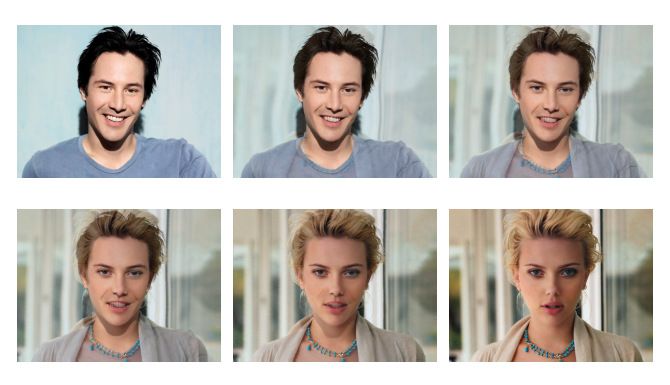
\includegraphics[scale=0.65]{imagenes/warping.png}
	\end{center}		
	\caption{Cross-dissolving con warping}
	\label{fig2}
\end{figure}

Organizamos esta exposici'on en cuatro partes. En primer lugar, proveemos un sencillo marco te'orico para comprender la matem'atica atr'as de esta t'ecnica. En segundo lugar, explicamos el algoritmo de Beier y Neely, con el m'aximo grado de detalle posible. En tercer lugar, desarrollaremos la vectorizaci'on realizada, contrastando esta implementaci'on contra la tradicional. Finalmente, presentamos los experimentos y, en base a ello, concluimos sobre la efectividad de la vectorizaci'on realizada.
	\section{Background matem'atico}

\subsection{Elementos de 'Algebra Lineal}

En esta secci'on hacemos breve repaso de las herramientas matem'aticas necesarias para comprender la raz'on de ciertos c'omputos involucrados en la t'ecnica de image morphing en la que nos basamos. Debemos notar, sin embargo, que la matem'atica es s'olo un elemento auxiliar para esta t'ecnica, y no aporta demasiado al entendimiento general de la misma. En esta sint'etica exposici'on de 'algebra lineal, no usaremos plena generalidad ni y en algunos casos priorizaremos la intuici'on antes que la rigurosidad.

Dado que la t'ecnica de Beier y Neely procesa a la imagen como un plano de dos dimensiones (y no maneja, por ejemplo, la profundidad de la imagen), hablaremos siempre en el contexto del $\mathbb{R}$-espacio vectorial $\mathbb{R}^2$. Durante todo este trabajo, las negritas min'usculas $\mathbf{x}$ ser'an vectores, y las it'alicas min'usculas $x$ ser'an escalares. Como el espacio vectores que estamos considerando es un conjunto de puntos del plano, usaremos los t'erminos \textit{punto} y \textit{vector} indistintamente.

Recordemos que el producto interno can'onico en $\mathbb{R}^2$ es la funci'on $\langle \cdot, \cdot\rangle_2: \mathbb{R}^2 \times \mathbb{R}^2 \to \mathbb{R}$ tal que

\[\langle (x_1, y_1), (x_2, y_2)\rangle_2 = x_1 x_2 + y_1 y_2\]

\noindent
Como todo producto interno, induce una norma, que es la funci'on $||\cdot||_2:\mathbb{R}^2 \to \mathbb{R}$ tal que

\[||\mathbf{p}||_2 = \sqrt{\langle \mathbf{p}, \mathbf{p}\rangle_2}\]

\noindent
que reescribiendo $\mathbf{p} = (x, y)$ queda

\[||(x, y)||_2 = \sqrt{x^2 + y^2}\]

\noindent
A su vez, toda norma induce una distancia entre vectores, que es la funci'on $d_2:\mathbb{R}^2 \times \mathbb{R}^2 \to \mathbb{R}$ tal que 

\[d_2(\mathbf{p}, \mathbf{q}) = ||\mathbf{p} - \mathbf{q}||_2\]

\noindent
y al reescribir $\mathbf{p} = (x_1, y_1)$ y $\mathbf{q} = (x_2, y_2)$ queda

\[d_2((x_1, y_1), (x_2, y_2)) = \sqrt{(x_1 - x_2)^2 + (y_1 - y_2)^2}\]

\noindent
que 'esta es la conocida distancia eucl'idea. En lo que sigue, y por simplicidad, notaremos $\langle \cdot, \cdot \rangle$, $||\cdot||$ y $d$ a las tres funciones anteriores.

A partir de la distancia entre vectores surge el concepto de distancia entre un vector y un subespacio. Recordemos que un subespacio no es m'as que un subconjunto de vectores que es, en s'i mismo, un espacio vectorial. Por ejemplo, en $\mathbb{R}^2$, las rectas que pasan por el origen son subespacios. La distancia entre un vector $\mathbf{p}$ y un subespacio $L$ es

\[d(\mathbf{p}, L) = \min\limits_{\mathbf{x} \in L} d(\mathbf{p}, \mathbf{x})\]

\noindent
Los subespacios que vamos a considerar son rectas por el origen, que son los 'unicos subespacios propios no nulos de $\mathbb{R}^2$, con lo cual vamos a estar calculando la distancia entre un punto y una recta. Es posible calcular f'acilmente esta distancia, y para esto vamos a caracterizar el 'unico punto del subespacio que realiza el m'inimo.

El concepto clave para dar con esta caracterizaci'on es el de \textit{proyecci'on ortogonal} de un vector sobre un subespacio. Supongamos que tenemos un punto $\mathbf{p}$ y una recta $L$, y tracemos la recta perpendicular $L^{\perp}$. El punto $\mathbf{p}$ se puede escribir como la suma de un punto $\mathbf{q} \in L$ y otro punto $\mathbf{r} \in L^{\perp}$. En la figura \ref{fig3} podemos ver la situaci'on.

\begin{figure}[H]
	\begin{center}
		%\includegraphics[scale=]{}
	\end{center}		
	\caption{}
	\label{fig3}
\end{figure}

\noindent
En este escenario, el punto $\mathbf{q}$ es la proyecci'on de $\mathbf{p}$ sobre el subespacio $L$, en la direcci'on de la recta ortogonal $L^{\perp}$. Esto es lo que se denomina, m'as sint'eticamente, proyecci'on ortogonal de $\mathbf{p}$ sobre $L$. Como indica la intuici'on, 'este es el punto de $L$ m'as cercano a $\mathbf{p}$, es decir que

\begin{equation*}
d(\mathbf{p}, L) = d(\mathbf{p}, \mathbf{q})
\label{eq_dist_1}
\end{equation*}

\noindent
Adem'as, esta distancia es exactamente la longitud del vector $\mathbf{r}$, con lo cual

\begin{equation*}
d(\mathbf{p}, \mathbf{q}) = ||\mathbf{r}||
\label{eq_dist_2}
\end{equation*}

Como $L$ es una recta, podemos escribir $L = \langle \mathbf{u} \rangle = \{\alpha \mathbf{u}: \alpha \in \mathbb{R}\}$ para cierto vector $\mathbf{u}$, un vector director de la recta. Como $\mathbf{q}$ es un punto de $L$, existe $u \in \mathbb{R}$ tal que $\mathbf{q} = u\mathbf{u}$. Este $u$ es el coeficiente que determina la posici'on de $\mathbf{q}$ sobre la recta $L$. Se puede demostrar que 

\begin{equation}
u = \frac{\langle \mathbf{p}, \mathbf{u} \rangle}{||\mathbf{u}||^2}
\label{eq_u}
\end{equation}


An'alogamente, si $L^{\perp} = \langle \mathbf{w} \rangle$ y $\mathbf{r} = w \mathbf{w}$, entonces

\[w = \frac{\langle \mathbf{p}, \mathbf{w}\rangle}{||\mathbf{w}||^2}\]

Como $L^{\perp}$ es la recta perpendicular a $L$, hay una fuerte relaci'on entre los vectores directores de ambas rectas. Si $\mathbf{u} = (x, y)$, llamamos $perp(\mathbf{u}) = (y, -x)$ al vector que se obtiene de rotar $\pi / 2$ radianes en sentido antihorario a $\mathbf{u}$. Se puede ver que $perp(\mathbf{u})$ es perpendicular a $\mathbf{u}$ y tiene la misma norma. Este vector $perp(\mathbf{u})$ resulta ser un director de $L^{\perp}$, con lo cual podemos poner $\mathbf{w} = perp(\mathbf{u})$, y por lo tanto

\begin{equation}
w = \frac{\langle\mathbf{p}, perp(\mathbf{u})\rangle}{||\mathbf{u}||^2}
\label{eq_ww}
\end{equation}

En definitiva, las ecuaciones \ref{eq_u} y \ref{eq_ww} caracterizan las proyecciones $\mathbf{q}$ y $\mathbf{r}$ en funci'on del punto proyectado $\mathbf{p}$ y un vector director $\mathbf{u}$ de la recta sobre la que se proyecta.

\subsection{Interpolaci'on Lineal}

\label{interp}

Dados dos puntos $(x_1, y_1)$ y $(x_2, y_2)$, existe una 'unica recta que los interpola. Si $x_1 \neq x_2$, esta recta es descripta por la f'ormula $y(x) = ax + b$, donde

\begin{align*}
a &= \frac{y_2 - y_1}{x_2 - x_1}\\
b &= y_1 - a x_1
\end{align*}

\noindent
Los puntos de la recta ser'an de la forma $(x, y(x))$.

Si $x_1 = x_2$, podemos expresar la recta sencillamente como $x(y) = x_1$, y sus puntos  son de la forma $(x(y), y)$.

Podemos expresar a ambas rectas, como una parametrizaci'on $\alpha: [0, 1] \to \mathbb{R}^2$, haciendo que la variable independiente var'ie entre los extremos de la interpolaci'on, a medida que el argumento $t$ de la parametrizaci'on $\alpha(t)$ var'ia de entre 0 y 1.

Si $x_1 \neq x_2$, esta parametrizaci'on tiene la forma $\alpha(t) = (x(t), y(x(t)))$, donde

\begin{align*}
x(t) &= (x_2 - x_1) t + x_1\\
y(x(t)) &= a(x_2 - x_1)t + ax_1 + b
\end{align*}

Si $x_1 = x_2$, la parametrizaci'on tiene la forma $\alpha(t) = (x(y(t)), y(t))$, donde

\begin{align*}
x(y(t)) &= x_1\\
y(t) &= (y_2 - y_1) t + y_1
\end{align*}

La expresi'on param'etrica tiene una gran ventaja respecto de la forma expl'icita (dejando una variable libre, mediante la cual se expresa la restante), que es que permite manejar los dos casos $x_1 = x_2$ y $x_1 \neq x_2$ de la misma manera, expresando, en ambos casos, las dos componentes de la parametrizaci'on como funciones lineales de $t$. Por el contrario, la dependencia entre las variables en la forma expl'icita cambia seg'un el caso, siendo $y$ dependiente de $x$ si $x_1 = x_2$, y $x$ dependiente de $y$ si $x_1 \neq x_2$.
	\section{Algoritmo de Beier y Neely}

\subsection{Metamorfosis dirigida por segmentos}

Para mapear las caracter'isticas de la imagen origen en las caracter'isticas de la imagen destino, esta t'ecnica utiliza segmentos dirigidos. A trav'es de ellos podemos indicar que todos los puntos sobre un sector de la imagen origen deben ser mapeados a cierto otro sector de la imagen destino. Estos segmentos establecen un campo de influencia en su entorno, de modo tal que todos los pixeles que se encuentren en estas inmediaciones ser'an mapeados al entorno del segmento destino asociado.

\subsection{Deformaci'on de una imagen}

Si bien estos pares de segmentos nos dan una idea de c'omo debe ser la transformaci'on, no es evidente el lugar exacto de la im'agen destino en el que debe ser mapeado cada pixel de la im'agen origen, ni tampoco c'omo deben moverse estos pixeles sobre las im'agenes intermedias, a lo largo de la deformaci'on.

¿C'omo construimos una im'agen intermedia? Cada una de 'estas estar'a compuesta por pixeles que provienen de la imagen origen y de la imagen destino. La pregunta es cu'ales son esos pixeles fuente.

Hay dos formas de mapear pixeles entre las im'agenes origen y destino, y la im'agen intermedia. La m'as intuitiva, aunque poco efectiva, es el mapeo hacia adelante (en ingl'es, \textit{forward mapping}), que consiste en mapear pixeles desde las im'agenes fuente (las im'agenes origen y destino) hacia la im'agen intermedia. Lo malo de esta t'ecnica es que podr'ian quedar pixeles de la im'agen intermedia sin pintar.

La alternativa es el mapeo hacia atr'as (en ingl'es, \textit{reverse mapping}) y consiste en, a contrapelo de lo anterior, mapear pixeles desde la im'agen intermedia, hacia los extremos. En otras palabras, para cada pixel de la imagen deformada, determina qu'e pixel de cada imagen fuente le corresponde. Esto asegura que cada pixel de la imagen deformada obtendr'a un color.

\begin{figure}[H]
	\begin{center}
		\input{imagenes/fig4.pdf_tex}
	\end{center}		
	\caption{Forward mapping y reverse mapping}
	\label{fig4}
\end{figure}

\subsection{Esquema general de la metamorfosis}

Fijados los pares de segmentos en la imagen origen y destino, interpolamos los extremos de cada uno de estos pares, de modo tal de determinar la ubicaci'on de estos segmentos en cada una de las im'agenes intermedias en la metamorfosis. En este trabajo optamos por interpolar linealmente, aunque bien podr'ia utilizarse otro m'etodo.

\begin{figure}[H]
	\begin{center}
		\input{imagenes/fig5.pdf_tex}
	\end{center}		
	\caption{Interpolaci'on de segmentos}
	\label{fig5}
\end{figure}

Para cada imagen intermedia a generar, determinamos las posiciones de los segmentos en dicha imagen. Luego, para cada pixel de esta imagen determinamos de qu'e pixel de la imagen original proviene, bas'andonos en la posici'on actual de los segmentos. Repetimos el proceso, ahora para determinar de qu'e pixel de la imagen destino proviene. Finalmente, hacemos una mezcla (en ingl'es, \textit{blending}) de los pixeles origen y destino calculados, como parte del cross-dissolving. Esta mezcla consiste en la suma ponderada, componente a componente RGB, de los pixeles involucrados, en la que el peso de cada componente depende del momento de la metamorfosis que estamos construyendo. Hacia el principio de la metamorfosis, el color del pixel original dominar'a, mientras que hacia el final, el color del pixel destino lo har'a.

\begin{figure}[H]
	\begin{center}
		\input{imagenes/fig6.pdf_tex}
	\end{center}		
	\caption{Construcci'on de una imagen intermedia}
	\label{fig6}
\end{figure}

\subsection{Transformaci'on con un 'unico segmento}

Supongamos por el momento que hay un 'unico segmento definido. En el contexto de la figura \ref{fig6}, ¿c'omo hacemos para encontrar la coordenada $\mathbf{x_{src}}$? Lo que haremos es encontrar la posici'on del punto $\mathbf{x}$ relativa al segmento dirigido $\mathbf{pq}$ y encontrar el pixel correspondiente a esta misma posici'on relativa pero con respecto al segmento dirigido $\mathbf{p_{src}q_{src}}$. Para esto, vamos a utilizar la proyecci'on de $\mathbf{x}$ sobre la recta que determina $\mathbf{pq}$, y sobre su ortogonal.

Lo primero que haremos es trasladar todo al origen, por lo que todos los c'omputos los haremos en t'erminos del punto $\mathbf{x} - \mathbf{p}$ y las rectas de directores $\mathbf{q} - \mathbf{p}$ y $\mathbf{q_{src}} - \mathbf{p_{src}}$. Por la ecuaci'on \ref{eq_u}, el coeficiente de la proyecci'on de $\mathbf{x} - \mathbf{p}$ sobre la recta $\langle \mathbf{q} - \mathbf{p} \rangle$ es

\begin{equation}
u = \frac{\langle \mathbf{x} - \mathbf{p}, \mathbf{q} - \mathbf{p} \rangle}{||\mathbf{q} - \textbf{p}||^2}
\label{eq_u_posta}
\end{equation}

\noindent
de modo tal que la proyecci'on es exactamente $u (\mathbf{q} - \mathbf{p})$, es decir, la proyecci'on se encuentra en el m'ultiplo $u$ del vector $\mathbf{q} - \mathbf{p}$. Luego,

\begin{equation}
u (\mathbf{q_{src}} - \mathbf{p_{src}})
\label{eq_qp}
\end{equation}

\noindent
es la proyecci'on asociada a $\mathbf{x_{src}}$, proporcional al segmento $\mathbf{p_{src}q_{src}}$. Notar que las proporciones se preservan porque la magnitud $u$ es una proporci'on. Intuitivamente, hemos determinado a qu'e \textit{altura} del segmento $\mathbf{p_{src}q_{src}}$ se encuentra $\mathbf{x_{src}}$.

Para determinar cu'an lejos se encuentra, vamos a usar la proyecci'on sobre el ortogonal $\langle \mathbf{q} - \mathbf{p} \rangle^{\perp}$. El coeficiente de la proyecci'on es, seg'un la ecuaci'on \ref{eq_ww},

\[w = \frac{\langle \mathbf{x} - \mathbf{p}, perp(\mathbf{q} - \mathbf{p}) \rangle}{||\mathbf{q} - \mathbf{p}||^2}\]

Podr'iamos usar este coeficiente para ubicar $\mathbf{x_{src}}$, aunque esto significar'ia que las proporciones tambi'en se preservan en la direcci'on ortogonal a $\mathbf{pq}$. Seg'un indican los creadores de la t'ecnica en su art'iculo, es m'as util \emph{no} mantener la escala en la direcci'on ortogonal al segmento. En otras palabras, la distancia del punto $\mathbf{x_{src}}$ a la recta $\langle \mathbf{q_{src}} - \mathbf{p_{src}} \rangle$ debe ser la misma que del punto $\mathbf{x}$ a la recta $\langle \mathbf{q} - \mathbf{p} \rangle$, sumado a que los puntos deben preservar su ubicaci'on con respecto a los segmentos, en el sentido de que o bien ambos puntos se encuentran a izquierda de los segmentos, o bien ambos se encuentran a derecha. Nosotros hemos seguido su consejo.

Notemos que podemos escribir la proyecci'on $w\hspace{0.1cm}perp(\mathbf{q} - \mathbf{p})$ como $\frac{\langle \mathbf{x} - \mathbf{p}, perp(\mathbf{q} - \mathbf{p}) \rangle}{||\mathbf{q} - \mathbf{p}||} \frac{perp(\mathbf{q} - \mathbf{p})}{||\mathbf{q} - \mathbf{p}||}$. Llamemos

\begin{equation}
v = \frac{\langle \mathbf{x} - \mathbf{p}, perp(\mathbf{q} - \mathbf{p}) \rangle}{||\mathbf{q} - \mathbf{p}||}
\label{eq_v_posta}
\end{equation}

\noindent
La clave es que, como $\frac{perp(\mathbf{q} - \mathbf{p})}{||\mathbf{q} - \mathbf{p}||}$ es unitario y tiene la direcci'on y el sentido de $perp(\mathbf{q} - \mathbf{p})$, entonces 

\begin{equation}
v \hspace{0.10cm} \frac{perp(\mathbf{q_{src}} - \mathbf{p_{src}})}{||\mathbf{q_{src}} - \mathbf{p_{src}}||}
\label{eq_qp_ort}
\end{equation}

\noindent
es una componente en direcci'on ortogonal a $\mathbf{p_{src}q_{src}}$ que preserva distancia y sentido, en la forma en que se indic'o en el p'arrafo anterior.

En definitiva, las expresiones \ref{eq_qp} y \ref{eq_qp_ort} determinan las componentes de $\mathbf{x_{src}} - \mathbf{p}$, de manera que

\begin{equation}
\mathbf{x_{src}} = u (\mathbf{q_{src}} - \mathbf{p_{src}}) + v \hspace{0.10cm} \frac{perp(\mathbf{q_{src}} - \mathbf{p_{src}})}{||\mathbf{q_{src}} - \mathbf{p_{src}}||} + \mathbf{p}
\label{eq_x_posta}
\end{equation}

\begin{figure}[H]
	\begin{center}
		\input{imagenes/fig7.pdf_tex}
	\end{center}		
	\caption{Transformaci'on con un 'unico segmento}
	\label{fig7}
\end{figure}

\noindent
Para calcular $\mathbf{x_{dst}}$, el procedimiento es el mismo, ahora utilizando el segmento $\mathbf{p_{dst}q_{dst}}$ en lugar de $\mathbf{p_{src}q_{src}}$.

Teniendo las coordenadas $\mathbf{x_{src}}$ y $\mathbf{x_{dst}}$, s'olo resta hacer el blending entre tales puntos para obtener los colores de $\mathbf{x}$. Para cada componente RGB $c$, ponemos

\begin{equation}
c(\mathbf{x}) = (1 - t) \hspace{0.1cm}c(\mathbf{x_{src}}) + t \hspace{0.1cm} c(\mathbf{x_{dst}})
\label{eq_blend}
\end{equation}

\noindent
donde $t \in [0, 1]$ es el tiempo transcurrido en la metamorfosis.

\subsection{Transformaci'on con m'ultiples segmentos}

En general, las metamorfosis en las que estemos interesados ser'an complejas y requerir'an m'as de un segmento. Cuando hay m'as de un segmento, cada punto no se ve afectado por un 'unico segmento cercano, sino por todos, que ejercen influencia en mayor o menor medida. Para determinar el pixel origen correspondiente a un punto $\mathbf{x}$, vamos a tomar cada uno de los segmentos de la imagen intermedia, y su segmento asociado en la imagen origen, y hacer el reverse mapping como si el segmento considerado fuera el 'unico. El procesamiento para el $i$-'esimo segmento, que llamamos $\mathbf{p}[i]\mathbf{q}[i]$, resultar'a en un punto $\mathbf{x}_{\mathbf{src}}[i]$, lo que significa que, seg'un $\mathbf{p}[i]\mathbf{q}[i]$, $\mathbf{x}$ se desplaza en $\mathbf{d}[i] = \mathbf{x}_{\mathbf{src}}[i] - \mathbf{x}$. Cada uno de estos desplazamientos tendr'a un peso, que ser'a inversamente proporcional a la distancia de $\mathbf{x}$ a $\mathbf{p}[i]\mathbf{q}[i]$, y directamente proporcional a la longitud de $\mathbf{p}[i]\mathbf{q}[i]$. El desplazamiento definitivo, con el que determinaremos $\mathbf{x_{src}}$, ser'a el promedio ponderado de estos desplazamientos parciales.

El peso que utilizaremos es

\begin{equation}
weight = \left(\frac{||\mathbf{q}[i] - \mathbf{p}[i]||^c}{a + d(\mathbf{x}, \mathbf{p}[i]\mathbf{q}[i])}\right)^b
\label{eq_weight}
\end{equation}

\noindent
donde $a$, $b$ y $c$ son constantes prefijadas. La constante $a$ cumple la funci'on de que la expresi'on no se indefina para los puntos que se encuentran sobre el segmento $\mathbf{p}[i]\mathbf{q}[i]$, por lo que se debe elegir apenas mayor que cero. La constante $c$ determina cu'an influyente es la longitud de un segmento, de modo tal que a valores grandes de $c$, m'as influencia tienen los segmentos largos. Finalmente, la constante $b$ indica cu'anto cae la fuerza de un segmento en funci'on de la distancia a la que se encuentra. Si $b$ es grande, cada punto ser'a afectado s'olo por los segmentos que est'an cerca. Notar que si $b$ es cero, todos los segmentos afectan a todos los pixeles en igual medida.

Para calcular la distancia $d(\mathbf{x}, \mathbf{p}[i]\mathbf{q}[i])$, podemos usar el mismo coeficiente $u$ calculado usando la f'ormula \ref{eq_u_posta}. Si $u \in [0, 1]$ entonces la proyecci'on de $\mathbf{x}$ cae sobre el segmento $\mathbf{p}[i]\mathbf{q}[i]$, y el punto de la proyecci'on realiza la distancia, y se puede ver que esta distancia es $|v|$, para el valor de $v$ calculado en la ecuaci'on \ref{eq_v_posta}. Si $u < 0$ entonces la proyecci'on cae en un punto que tiene sentido contrario al segmento, por lo que la distancia se realiza sobre el extremo $\mathbf{p}[i]$, y vale $||\mathbf{x} - \mathbf{p}[i]||$. Finalmente, si $u > 1$, la distancia se realiza sobre el otro extremo $\mathbf{q}[i]$, y vale $||\mathbf{x} - \mathbf{q}[i]||$.

Terminamos esta explicaci'on presentando el algoritmo completo. El algoritmo \ref{algo1} es el encargado de, dado un pixel $\mathbf{x}$, encontrar el pixel $\mathbf{x'}$ correspondiente en una imagen fuente. En otras palabras, calcula $\mathbf{x_{src}}$ o $\mathbf{x_{dst}}$ seg'un se use los segmentos de la imagen origen o los de la imagen destino, respectivamente. El algoritmo \ref{algo2} es la transformaci'on completa.

%\newpage

\begin{algorithm}
\DontPrintSemicolon

\SetKwInOut{input}{Input}
\SetKwInOut{output}{Output}
\SetKwInOut{signature}{Signatura}

%\signature{\textsc{Compute-Source-Point}($\mathbf{x}$)}
\input{$\mathbf{x}$ pixel de la imagen intermedia\\$\mathbf{p}[]\mathbf{q}[]$ segmentos de la imagen intermedia\\
$\mathbf{p'}[]\mathbf{q'}[]$ segmentos de la imagen fuente}

\output{$\mathbf{x'}$ pixel de la imagen fuente}

%\output{}
$\mathbf{d\_{sum}} \gets (0, 0)$\;
$weight\_sum \gets 0$\;
Sea $s$ la cantidad de segmentos\;
\For{$i \gets 1$ \KwTo $s$}{
	Calcular $u$ y $v$ en base a $\mathbf{p}[i]\mathbf{q}[i]$ y $\mathbf{x}$ (ecuaciones \ref{eq_u_posta} y \ref{eq_v_posta})\;
	Calcular $\mathbf{x'}[i]$ en base a $u$, $v$, $\mathbf{p'}[i]\mathbf{q'}[i]$ y $\mathbf{p}[i]$ (ecuaci'on \ref{eq_x_posta})\;
	$\mathbf{d}[i] \gets \mathbf{x'}[i] - \mathbf{x}$\;
	Calcular $weight$ en base a $\mathbf{p}[i]\mathbf{q}[i]$ y $\mathbf{x}$ (ecuaci'on \ref{eq_weight}) \;
	$\mathbf{d\_{sum}} \gets \mathbf{d\_{sum}} + weight * \mathbf{d}[i]$\;
	$weight\_sum \gets weight\_sum + weight$\;
}

$\mathbf{x'} \gets \mathbf{x} + \mathbf{d\_{sum}}/weight\_sum$\;
\Return $\mathbf{x'}$\;
\caption[]{C'omputo de pixel fuente}
\label{algo1}
\end{algorithm}

\begin{algorithm}
\DontPrintSemicolon

\SetKwInOut{input}{Input}
\SetKwInOut{output}{Output}
\SetKwInOut{signature}{Signatura}

%\signature{\textsc{Compute-Source-Point}($\mathbf{x}$)}
\input{Imagen origen\\Imagen destino\\
$\mathbf{p_{src}}[]\mathbf{q_{src}}[]$ segmentos de la imagen origen\\
$\mathbf{p_{dst}}[]\mathbf{q_{dst}}[]$ segmentos de la imagen destino}

%\output{}
Sea $s$ la cantidad de segmentos\;
\For{$i \gets 1$ \KwTo $s$}{
	Calcular la interpolaci'on lineal de $\mathbf{p_{src}}[i]$ y $\mathbf{p_{dst}}[i]$ de forma param'etrica\;
	Calcular la interpolaci'on lineal de $\mathbf{q_{src}}[i]$ y $\mathbf{q_{dst}}[i]$ de forma param'etrica\;
}

\For{$t$ corriendo entre 0 y 1}{
	\ForEach{p'ixel $\mathbf{x}$}{
		Calcular $\mathbf{x_{src}}$ en base a $\mathbf{x}$, las interpolaciones en tiempo $t$ y los segmentos de la imagen origen (algoritmo \ref{algo1})\;
		Calcular $\mathbf{x_{dst}}$ en base a $\mathbf{x}$, las interpolaciones en tiempo $t$ y los segmentos de la imagen destino (algoritmo \ref{algo1})\;
		Colorear $\mathbf{x}$ mezclando $\mathbf{x_{src}}$ y $\mathbf{x_{dst}}$ (ecuaci'on \ref{eq_blend})\;
	}
	Escribir la im'agen intermedia\;
}
\caption[]{Metamorfosis}
\label{algo2}
\end{algorithm}

\newpage

En el algoritmo \ref{algo2} no est'a especificada la forma en que $t$ toma valores entre 0 y 1. En la pr'actica, esto est'a determinado por la cantidad de im'agenes intermedias que queremos que compongan a la metamorfosis. Si llamamos $f$ a la cantidad total de im'agenes que componen a la metamorfosis (es decir, la imagen origen, m'as las im'agenes intermedias, m'as la imagen destino), entonces $t$ tomar'a los valores $i / (f - 1)$, para $i = 0, \dots, f -1$, en ese orden.

\subsection{Complejidad temporal}

El algoritmo \ref{algo1} tiene un costo $O(s)$, puesto que el ciclo 4-11 se ejecuta $s$ veces, y cada una de sus operaciones es $O(1)$.

Las l'ineas 2 a 5 del algoritmo \ref{algo2}, en las cuales se computan las interpolaciones, cuestan $O(s)$ en total, puesto que son $2s$ interpolaciones en total y cada una cuesta $O(1)$, como se puede ver en la secci'on \ref{interp}. Los ciclos anidados 6-13 se ejecutan $f \times w \times h$ veces, donde $w$ es el ancho de las im'agenes y $h$ es el alto. Las l'ineas 8 y 9 son $O(s)$ cada una, mientras que la l'inea 10 es $O(1)$. Por lo tanto, el ciclo 6-13 es $O(f \times w \times h \times s)$ y, en definitiva, 'este es el costo del algoritmo.
	\section{Vectorizaci'on}

En los algoritmos \ref{algo1} y \ref{algo2} se puede ver que t'ecnica se compone de varias partes, claramente divididas. En primer lugar aparece el c'omputo de las interpolaciones. Luego, tenemos la metamorfosis propiamente dicha, etapa en la que se construye cada una de las im'agenes intermedias. Para cada una de ellas, se itera sobre todos los pixeles, y se realizan dos tipos de operaciones: reverse mappings y blending.

Dado que la cantidad de segmentos $s$ suele ser peque\~{n}a, se decidi'o no vectorizar el c'omputo de las interpolaciones. El blending tampoco fue vectorizado, puesto que, suponiendo que tenemos varios p'ixeles de la imagen origen y destino que mezclar, es muy probable que no ocupen posiciones consecutivas, forzando a la realizaci'on de m'ultiples lecturas de memoria necesarias para obtener las componentes RGB de tales pixeles. Por esta raz'on, el 'unico c'omputo en paralelo posible aqu'i ser'ia la cuenta de la ecuaci'on \ref{eq_blend}. Si bien esto podr'ia significar una ganancia de tiempo, es despreciable respecto del costo en que incurrimos al realizar los accesos a memoria, por lo que decidimos no vectorizarlo.

En donde s'i exist'ia una gran posibilidad de vectorizaci'on, es en el reverse mapping, es decir, el algoritmo \ref{algo1}, que tiene la caracter'istica deseable de branching casi inexistente. El 'unico momento en que debe tomar decisiones es al calcular la distancia $d(\mathbf{x}, \mathbf{p}[i]\mathbf{q}[i])$, en la l'inea 8.

La vectorizaci'on de este algoritmo logra computar, para una serie de cuatro pixeles $\mathbf{x}[0]$, $\mathbf{x}[1]$, $\mathbf{x}[2]$, $\mathbf{x}[3]$, el pixel fuente $\mathbf{x'}[0]$, $\mathbf{x'}[1]$, $\mathbf{x'}[2]$, $\mathbf{x'}[3]$ correspondiente a cada uno. La idea atr'as de esta implementaci'on es tomar todas las magnitudes computadas en el algoritmo est'andar ($u$, $v$, las coordenadas de todos los vectores involucrados, etc.), y disponer cada una en un registro XMM distinto. De esta forma, cada registro XMM contiene cuatro valores de una misma magnitud, correspondientes al procesamiento simult'aneo de los cuatro pixeles. En definitiva, esta vectorizaci'on puede pensarse como la ejecuci'on simult'anea de cuatro instancias del algoritmo \ref{algo1}, a trav'es de registros XMM.

Es cuatro es la cantidad de pixeles que se pueden procesar al mismo tiempo, debido a que todas las magnitudes involucradas son n'umeros de punto flotante de precisi'on simple, que tienen 4B de longitud, mientras que los registros XMM tienen 16B de longitud. Todos los c'omputos fueron realizados con representaci'on de punto flotante de dicha precisi'on.
	\section{Experimentaci'on}

\subsection{Resultados}

Comparamos una implementaci'on en C, con la vectorizada. Para esto, tomamos dos imagenes de tama\~{n}o $1024 \times 768$, y trazamos 44 segmentos sobre cada una de ellas. En la figura \ref{fig8} se puede ver la metamorfosis utilizando los 44 segmentos.

\begin{figure}[H]
	\begin{center}
		%\includegraphics[scale=]{}
	\end{center}		
	\caption{Metamorfosis empleada para benchmarking}
	\label{fig8}
\end{figure}

Para la comparaci'on, decidimos dejar fija las im'agenes origen y destino, es decir que $w = 1024$ y $h = 768$, fijar la cantidad de frames de la metamorfosis en $f = 100$, y variar la cantidad de segmentos $s$ utilizados. Esta elecci'on se basa en que el par'ametro $s$ es el que determina la intensidad del c'omputo de cada una de las llamadas individuales a la implementaci'on del algoritmo \ref{algo1}, que es la pieza que hemos vectorizado. Los par'ametros $f$, $w$ y $h$ solamente marcan cu'antas veces se llama a ese procedimiento.

Para cada una de las implementaciones, y variando $s \in \{0, 5, 10, 15, 20, 25, 30, 35, 40\}$, medimos el tiempo de ejecuci'on total, de todo el algoritmo \ref{algo2}. Esto incluye el overhead que impone en framework utilizado para el manejo de video, para la creaci'on de un frame sobre el que trabajamos a lo largo de todo el proceso, y su escritura en el video, al finalizar cada iteraci'on. Como se puede ver en los tiempos de ejecuci'on para $s = 0$, experimento en el que s'olo escribimos sobre el video, casi sin realizar c'omputos en el algoritmo \ref{algo1}, este overhead es despreciable respecto del resto del procesamiento.

En la figura \ref{fig9} presentamos los resultados de la comparaci'on. Ambas versiones fueron compiladas con el flag de optimizaci'on -O3. Como estamos variando 'unicamente $s$, los gr'aficos de los tiempo de ejecuci'on son, como se espera,  rectas, cuya pendiente es proporcional a $f \times w \times h$.

\begin{figure}[H]
	\begin{center}
		%\includegraphics[scale=]{}
	\end{center}		
	\caption{Comparaci'on C vs. SIMD}
	\label{fig9}
\end{figure}

Una cuenta permite ver que, en promedio, la implementaci'on SIMD es 25 veces m'as r'apida que la versi'on en C, lo cual es una diferencia m'as que notable.

\subsection{An'alisis}

En general, al vectorizar procedimientos obtenemos ganancias m'ultiplo de la cantidad de datos procesados al mismo tiempo. Sin embargo, en este caso, la vectorizaci'on supera ampliamente esa expectativa, al ser 25 veces m'as r'apida, pese a que cada ejecuci'on procesa s'olo 4 pixeles en paralelo. En busca de una explicaci'on para este fen'omeno, comparamos con lupa ambas implementaciones.

La implementaci'on con extensiones SIMD tiene dos caracter'isticas remarcables, directamente relacionadas con su performance:

\begin{itemize}
	\item \textbf{Casi todas las magnitudes involucradas se mantienen, todo el tiempo, en registros.} Esto permite evitar accesos a memoria, que son hasta 100 veces m'as costosos que los accesos a registros, en el caso de un cache miss.
	\item \textbf{Todas las funciones auxiliares est'an implementadas en forma de macros.} Si bien esto permite reducir el overhead de una implementaci'on que usa etiquetas e instrucciones \texttt{call}, la motivaci'on verdadera fue hacer la programaci'on m'as sencilla, puesto que, en el intento de mantener la mayor'ia de los datos en registros, 'estos deb'ian ser manipulados cuidadosamente. Utilizando macros podemos decidir exactamente qu'e registros queremos que sean utilizados por una rutina.
\end{itemize}

Ambas elecciones tienen desventajas. Por un lado, al intentar explotar al m'aximo la utilizaci'on de los registros, se hace mucho m'as complicada la programaci'on, al ser limitada la cantidad de registros que tenemos a nuestra disposici'on. Sortear este problema es simplemente una cuesti'on de planificar bien el programa. Por otro lado, la utilizaci'on de macros tiene dos desventajas. Primero, no es posible una utilizaci'on din'amica de ese pedazo de c'odigo, en el sentido de que cada llamada a la macro replicar'a su c'odigo, haciendo que el c'odigo objeto sea mucho m'as largo. En nuestro caso, el c'odigo objeto de la vectorizaci'on consta de algunos cientos de l'ineas, de modo que, en este caso, 'esto no resulta una verdadera contra. En segundo lugar, no es posible debuggear las l'ineas que componen a la macro, haciendo m'as dif'icil la detecci'on y correcci'on de errores.

Para realizar una fiel comparaci'on contra el programa C, realizamos un dump del c'odigo objeto de esta implementaci'on. La primer observaci'on que hicimos, es que la cantidad neta de l'ineas de la versi'on C del reverse mapping y todas las funciones auxiliares utilizadas, es de 650 l'ineas aproximadamente, mientras que la versi'on SIMD tiene alrededor de 350. Si bien un programa m'as compacto no es necesariamente mejor, en este caso es tenemos 350 l'ineas que fueron cuidadosamente pensadas, contrariamente a las 650 elaboradas por un compilador, lo cual podr'ia indicar que la mano humana est'a haciendo diferencia.

En este sentido, notamos que hay auxiliares del dump de C que son sorprendentemente complejas, especialmente las funciones \texttt{add} y \texttt{subtract}, que se encargan de sumar y restar vectores respectivamente. La versi'on SIMD de \texttt{add} se compone de las siguientes dos instrucciones:

\begin{verbatim}
addps xmm0, xmm2
addps xmm1, xmm3
\end{verbatim}

\noindent
donde \texttt{xmm0} y \texttt{xmm2} contienen las coordenadas $x$ de los vectores a sumar, y \texttt{xmm1} y \texttt{xmm3} las coordenadas $y$. El c'odigo original de la versi'on C es el siguiente:

\begin{verbatim}
point add(point a, point b) {
    point res;
    res.x = a.x + b.x;
    res.y = a.y + b.y;
    return res;
}
\end{verbatim}

\noindent
mientras que su dump es:

\begin{verbatim}
movq   QWORD PTR [rsp-0x38],xmm0
mov    rdx,QWORD PTR [rsp-0x38]
movq   QWORD PTR [rsp-0x38],xmm1
mov    rax,QWORD PTR [rsp-0x38]
mov    rcx,rdx
mov    DWORD PTR [rsp-0x10],edx
shr    rcx,0x20
mov    rsi,rax
mov    DWORD PTR [rsp-0xc],eax
mov    QWORD PTR [rsp-0x38],rcx
shr    rsi,0x20
movss  xmm3,DWORD PTR [rsp-0x38]
mov    QWORD PTR [rsp-0x28],rsi
movss  xmm2,DWORD PTR [rsp-0x10]
addss  xmm3,DWORD PTR [rsp-0x28]
addss  xmm2,DWORD PTR [rsp-0xc]
movss  DWORD PTR [rsp-0x38],xmm3
mov    rdx,QWORD PTR [rsp-0x38]
movss  DWORD PTR [rsp-0x10],xmm2
mov    eax,DWORD PTR [rsp-0x10]
shl    rdx,0x20
or     rax,rdx
mov    QWORD PTR [rsp-0x38],rax
movq   xmm0,QWORD PTR [rsp-0x38]
ret    
nop    WORD PTR cs:[rax+rax*1+0x0]
\end{verbatim}
	\bibliographystyle{plain}
	\bibliography{informe}
\end{document}
